%% --------- SRM - make sure they know this is what I did
\chapter{Sparse Reachable Map Velocity Space Inverse Kinematics}\label{sec:srm}
		%\begin{center}
\large\bf{Abstract:}
\end{center}
\normalsize

\bf{
\noindent The degrees of freedom (DOF) of robots and complex systems have been increasing increasing exponentially since the early 20th century.
Today it is common place for complex control systems to have 40 DOF. 
This number is projected to be 70 DOF by the year 2020.
Robots with high DOF allows for complex tasks such as tool manipulation, greater human-robot interaction and agile full-body locomotion.
More DOF require greater attention to local communication delays, bandwidth, system configuration and stability.
In addition different tasks being performed by separate parts of the robot in tandem bring on greater issues including controller timing and priorities.
The increase in DOF on single system requires that the traditional methods of controller design be re-examined.

\noindent This dissertation describes a Unified Algorithmic Framework for High Degree of Freedom Complex Systems and Humanoid Robots that allows a user to develop controllers using a three tier infrastructure.
The Unified Algorithmic Framework called Hubo-Ach is a multi-process based system that allows for robust multi-rate simultaneous control and seamless implementation between virtual, miniature, and full-size robots with no modification.
The three tier infrastructure provides different levels of cost to entry and testing.
Examples of this field tested framework functioning on simulated, miniature, and full-size high DOF robots is given as well as validation by external researchers.
}




		%The number of degrees of freedom (DOF) of control systems are increasing exponentially since the early 20$^{th}$ century.
Today it is common place for complex control systems to have 40 DOF. 
This number is projected to be 70 DOF by the year 2020 (see Section~\ref{sec:numdof}).
\textit{The increase in DOF on single system requires that the traditional methods of controller design needs to be re-examined}.
High DOF complex system, or robots, allow for complex tasks such as using human tools and interfaces \cite{lofaroRAM2013,lofaroTePRA2013HuboAch,lofaroTePRA2013Valve,gtechIK}, playing music \cite{lofaroEURASIP2011, 6094987,lofaroIASTED2011,5686847} and other complex tasks \cite{lofaroHumanoids2012,lofaroGamesRobot,tepraLadder2013}.

\cite{orocos-gadeyne-ijrr2005}
\cite{multiPC-arch-1185243}
\cite{multi-thread-robot-5602743}
\cite{multi-thread-snake-1541141}
\cite{multi-thread-5524083}
\cite{openHRP}
\cite{Webots}




Due to the nature of these highly redundant complex electrical mechanical system it is common to have multiple different controllers running in tandem.  
Different controllers are needed when the system is in different states or doing different tasks or performing multiple tasks at the same time.
Combining these controllers is a problem in complex system.
This problem is hard when each controller has different frequencies, timing requirements (asyncronous vs. syncronous), latency restrictions, newest state data ie smore important then older state data and most basic of all languages the controller is written in.
This is especially true for complete and complex autonomous systems.
I define a complete and complex autonomous system as an electro mechanical mechanism with high degree of freedom (DOF) that is capable of making its own decisions through the use of sensor data processed by its artificial intelligence (AI).
The combination of high DOF and the requirement for autonomy makes the work space broad and controllers complex.
The overarching question becomes; What is the control system structure for a complete and complex autonomous systems with high DOF, a multitude of sensors, AI performing high-level and low-level tasks all while keeping a stable system structure conducive to collaborative work?
Current methods of solving the problem of controller synchrony and latest state data is to keep your critical control elements in the primary control loop.
Inter-process communication (IPC) and/or network sockets to communicate between the high level and low level processes even if written in different languages.
The majority of IPC have the problem of \textit{head of line} blocking (HOL) which means you must read the older data in a buffer before you read the newest data.
In the computer science field this is not a problem because all data being intact is typically desired.  
In the field of robotics and control the most recent state data is more important to a real-time control system to act on.
This thesis shows that by expanding on the idea of multi-process controllers connected to high-speed low-latency IPC you can create a \textit{robot layer} on a computer platform that will allow low-level controllers to run in separate processes while still allowing them access to the most recent data as the priority.
The new technical idea is the \textit{robot layer}, a control layer that allows external processes to run like normal and not deal with the specifics of the given robot system.
The robot system can be replaced by a simulated system without any of the processes needing to be modified or even know of the change.
This allows more mature controllers to be easily interfaced with this system without modifying control rates or timing.
This \textit{robot layer} must be:
\begin{itemize}
\item Have a IPC latency much less then that of the robot's inherent sampling period $t_{ipc}<<T_{r}$
\item Allow for command rates much slower then the inherent sampling period $T_{slow}>>T_{r}$
\item Allow for command rates much faster then the inherent sampling period $T_{fast}<<T_{r}$
\item Allow for arbitrary command rates.
\item Allow for real-time and non-real-time controllers to command actuators
\item Allow for all processes to have access to the newest data first
\item Allow for no more then one rt time step delay between command and robot actuator retrieval
\item Commanded such that it is for an arbitrary robotic actuator.
\item Triggering for process synchronization
\item Triggering for simulator synchronization and holding
\end{itemize}
We can succeed now not only because the bleeding edge technology allows for the fast enough communication between processes with access to the latest data.

Results are measured quantitatively and qualitatively.
Data showing proper loop rates, timings, controller implementation, simulation connections etc. show the viability of the system.
User survey shows methodology is sound, useful, and practical.





My Thesis shows is that a multi-process control structure coupled with the proper timing mechanisms is conducive to answering these questions.
It is shown with physical experiments and the creation of Hubo-Ach\cite{lofaroRAM2013}; a fully functional Sim-Time and Real-Time control system for complete and complex autonomous systems.

Through experimentation I prove my control system is a viable way of controlling complete and complex autonomous system and still be conducive to collaborative work.  
A road map of how my research has taken me to my thesis is shown in Section~\ref{sec:roadmap}.
As proof of viability I show the basic structure of my system \textit{Hubo-Ach} in Section~\ref{sec:hubo-ach}.  
I give step by step examples in Section~\ref{sec:simpleExamples}.
Section~\ref{sec:simulator} shows how we can move from real-time to using a simulated version of the platform in simulation time without having to change the controller.
Section~\ref{sec:task} describes the experiment which consists of making the robot preform an advanced task that pulls together visual, kinematic, path planning and other controllers together using this one system.
The techniques used stem from my contributions in Section~\ref{sec:contributions}.
Section~\ref{sec:results} shows the results of the experiment thus show the viability of the system.
Lastly Section~\ref{sec:conclusion} discusses the results of the work and the future of this system.

Before I continue it is important to note that my work has already been validated by my pears because:
\begin{itemize}
\item It was chosen to be the primary control system for the DARPA Robotics Challenge Track-A Team DRC-Hubo, Section~\ref{sec:drc}.
\item It is being used in the NSF-MIRR project\footnote{NSF-MIRR: Major Research Infrastructure Recovery and Reinvestment (MIRR) \#CNS-0960061 sponsored by the the U.S. National Science Foundation (NSF)}.
\item It is currently being used by MIT, WPI, Purdue, Ohio State, Swarthmore College, Georgia Tech, and Drexel University.
\end{itemize}

For the remainder of this document the complete and complex autonomous systems that I will be referring to are robots.
The majority of examples given will be in reference to humanoid robotics and the Hubo2+ (KHR-4+) platform.
The Hubo platform is described in Section~\ref{sec:hubo}.





		\section{RELATED WORK}

Low degree of freedom throwing machines/robots are common.  
%Typical throwing robots have between one and three degrees of freedom (DOF) \cite{509405,Lynch97dynamicnonprehensile,5152525,509335,springerlink:10.1007/s10015-006-0401-0}.  
All of these mechanisms are limited to throwing in a plane.   
Sentoo et al.\cite{4651142} achieved an end-effector velocity of 6.0 m/s and can throw in $R^3$ space using it's Barret Technology Inc 4-DOF arm with a $360^o$ rotation base yaw actuator.  
These low degree of freedom throwing robots are either physically attached/planted to the mechanical ground or have a base that is significantly more massive then the arm.  

%\cite{5686315,JooH2011438}
Kim et al. \cite{JooH2011438} takes the research to the next level with finding optimal overarm and sidearm throwing motions for a high degree of freedom humanoid computer model.  
The model consists of 55-DOF and is not fixed to mechanical ground or a massive base.  
Motor torques are then calculated that both allows for a sidearm or overarm throw and continuously satisfies the zero-moment-point stability criteria \cite{4309277}.  

%Kim was able to receive a maximum flight time of 2.784s and 3.711s for overarm and sidearm throws respectively.



		\section{Methodology}\label{sec:methodology}
%\subsection{Balance and Stability}\label{sec:sec:balance}
Each of the methods used have to be stable through the motion in order for the system to be stable (i.e. not to fall down).  
The well known zero-moment-point (ZMP) criteria is what each method must adhere to in order to stay statically stable\cite{Vukobratovic19721}.  
To handle perturbation an active balance controller was added.  
The active balance controller is applied on top of the pre-defined trajectories.  
Hubo is modeled as a single inverted pendulum with the center of mass (COM) located at length $L$ from the ankle.  
The compliance of the robot is composed of a spring $K$ and a damper $C$, see Fig.~\ref{fig:invPen}.  
An IMU located at the COM gives the measured orientation.

\begin{figure}[t]
  \centering
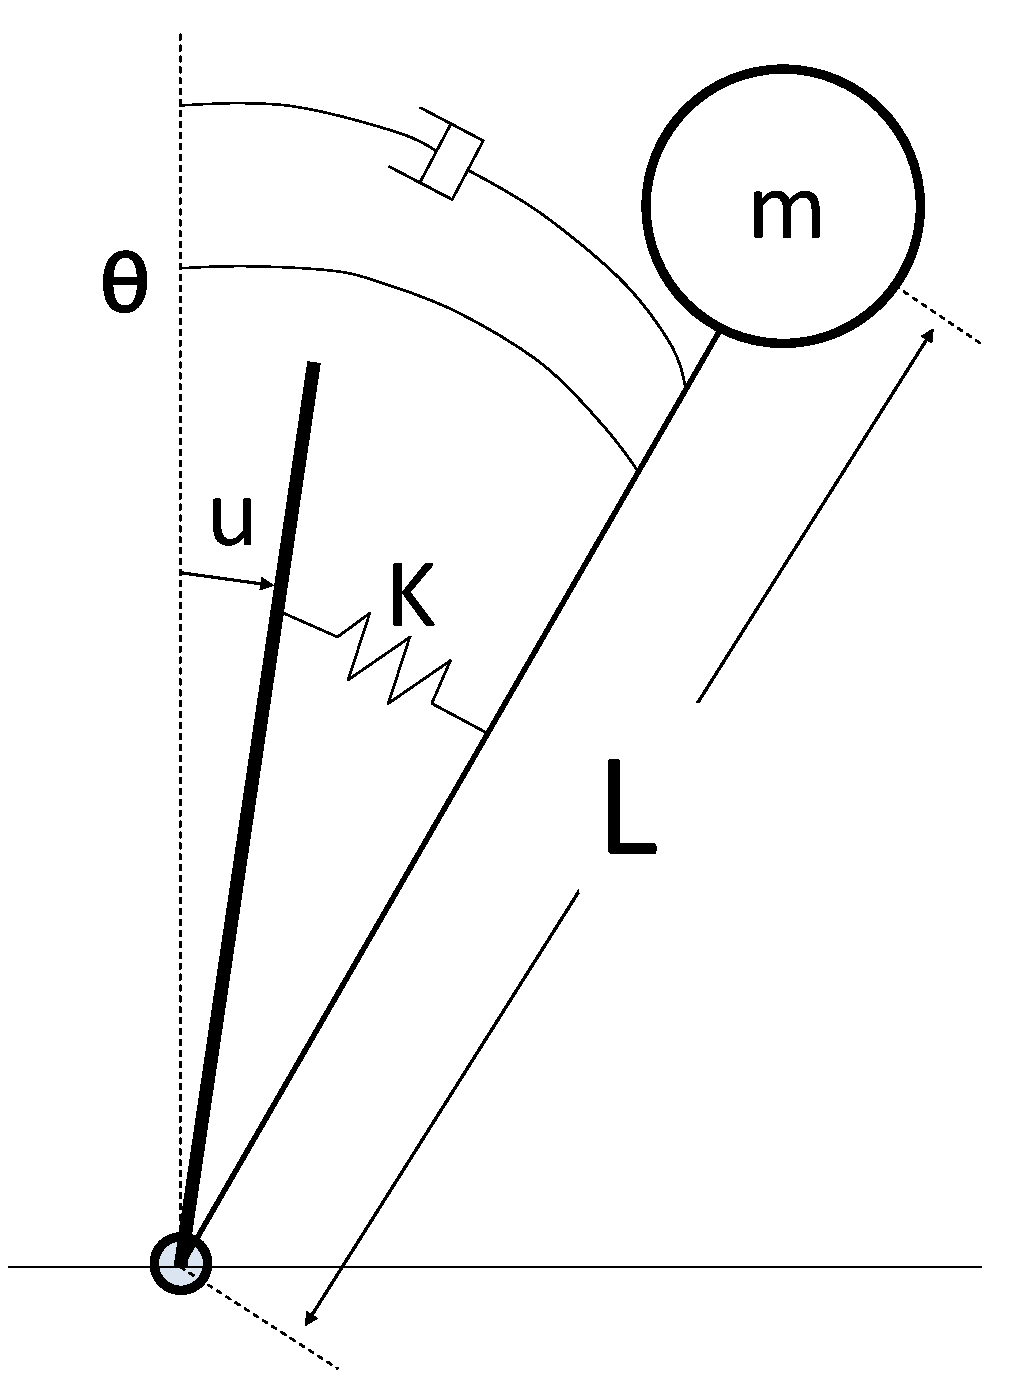
\includegraphics[width=0.4\columnwidth]{./pix/invPen3.pdf}
  \caption{Hubo modeled as a single inverted pendulum with COM located a distance $L$ from }
  \label{fig:invPen}
\end{figure}

The dynamic equation of the simplified model is assumed to be the same in both the sagittal and coronal plane.

\begin{equation}
mL^2\ddot{\theta}+C\dot{\theta}-K\theta = Ku
\end{equation}

This can be linearized and made into the transfer function:

\begin{equation}
%G(s) = \frac{\Theta(s)}{U(s)} = \frac{K}{ mL^2s^2 + Cs + (K - mgL)}
G(s) = \frac{\Theta(s)}{U(s)} = \frac{\frac{K}{mL^2}}{s^2+\frac{C}{mL^2}s + \frac{K-mgL}{mL^2}}
\end{equation}

Prior work on the model and controller for the Hubo by Cho et. al. calculated K=753 $\frac{Nm}{rad}$ and C=18 $\frac{Nm}{sec}$ using the free vibration response method\cite{5379574}.


\begin{figure}[ht]
  \centering
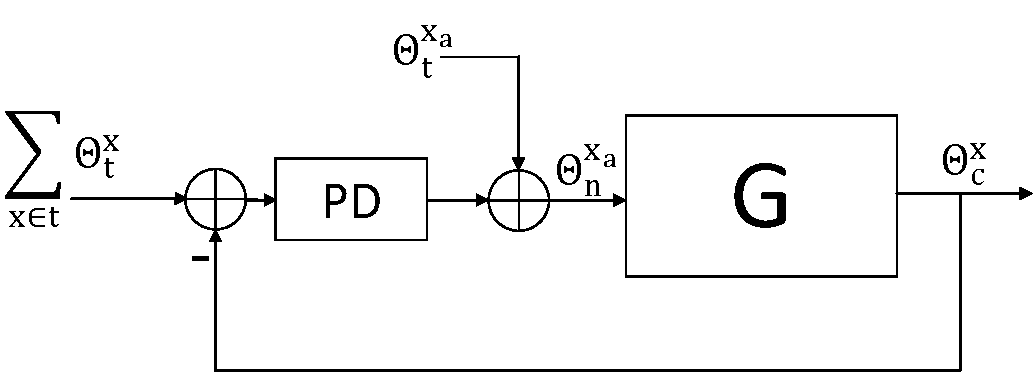
\includegraphics[width=0.8\columnwidth]{./pix/blockDiagram3.pdf}
  \caption{Block diagram of the balance controller used to balance Hubo in this work.}
  \label{fig:ctrlBlockDiagram}
\end{figure}

The control law is as follows
%ffFor the ankle roll (in the coronal plane) it is always assumed that the desired orientation of the COM is zero degrees.  Thus the roll of the IMU is taken as the error.

\begin{equation}
\theta_n^{x_a} = \theta_t^{x_a} + \left(K_p^x+sK_d^x\right)\left(\sum\limits_{x \in t} \theta_{t}^x - \theta_{c}^x\right)
%\theta_{n}^x = \theta_{t}^x + \left(K_p^x+sK_d^x\right)\left(\sum \theta_{t}^x - \theta_{c}^x\right)
%\theta_{n}^x = \theta_{t}^x + (K_p^x+sK_d^x)(\sum \theta_{t}^x - \theta_{c}^x)
%\theta_{new} = \theta_{traj} + (K_p+sK_d)(\sum \theta_{leg} - \theta_{IMU})
\end{equation}

Where $\theta_t$ is the desired trajectory of the lower body (pitch or roll), $x$ denotes pitch or roll and $x_a$ denotes pitch or roll on the ankle.  $\theta_{c}$ is the orientation of the center of mass in the global frame.  $\theta_n$ is the resulting trajectory.  $K_p$ and $K_d$ are the proportional and derivative gains.  The resulting control allows for a stable stance even with perturbations from upper body motions.



		%% split trapozoidal motion profile into another section example


\section{Final Design}\label{sec:finalDesign}
	The final goal is the have an end-effector velocity of 9.47 $\frac{m}{s}$ at $45^o$.  
The key-frame method was tested to throw at 4.8 $\frac{m}{s}$.  
To increase the end-effector velocity the upper body motion was kept unchanged but the lower body added a stepping motion with its legs.
The stepping motion consists of lifting the left foot up, pushing forward with the right and move the left forward 10 cm.  
Stepping with your non-dominant foot, and pushing with the dominant, when throwing overhand is common practice to increase the distance you can throw a ball.  
Jaemi Hubo throws with its right hand and steps with its left.  
This increased the end-effector velocity from 4.8 $\frac{m}{s}$ to 7.1 $\frac{m}{s}$.
Fig.~\ref{fig:hubo-step} shows the stepping motion of the robot.

\begin{figure}[t]
  \centering
\includegraphics[width=0.8\columnwidth]{./pix/throwPractice.png}
  \caption{Hubo stepping 10 cm up and forwards increasing the end effector velocity by 2.3 $\frac{m}{s}$.}
  \label{fig:hubo-step}
\end{figure}

The addition of pushing off with the right foot and stepping forward introduced two problems.  1) The ZMP criteria is not satisfied throughout the motion and 2) the right foot would slip when pushing its body forward.  
To avoid slip \textit{hook and loop} was paced on the bottom of the right foot (non-dominant) and on the throwing platform.  
This did not permanently attach the robot to the platform but it did allow for more friction between the foot and the ground.
This allowed the balancing controller to function adequately for the short step and maintain stability.
The platform was added to ensure a more consistent ground for the robot to balance on than the baseball field can inherently provide.

\begin{figure}[t]
  \centering
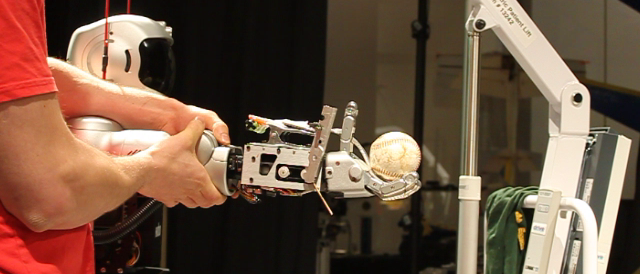
\includegraphics[width=0.4\columnwidth]{./pix/arm0.png}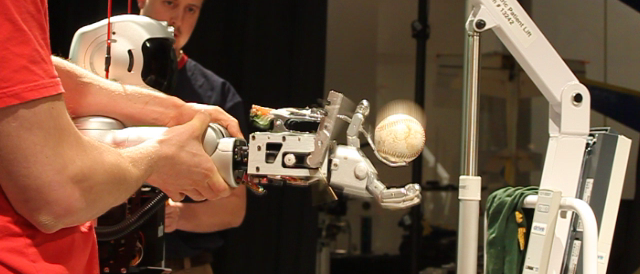
\includegraphics[width=0.4\columnwidth]{./pix/arm1.png}
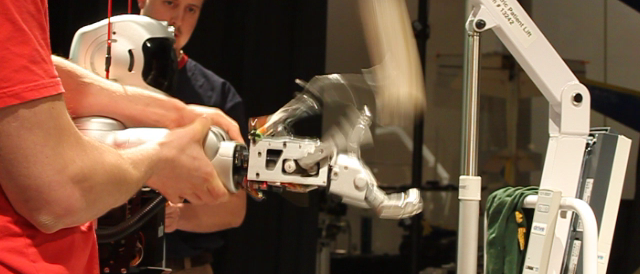
\includegraphics[width=0.4\columnwidth]{./pix/arm2.png}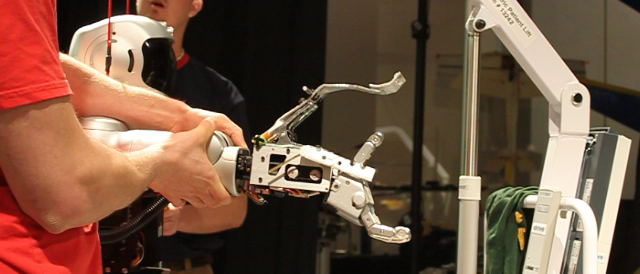
\includegraphics[width=0.4\columnwidth]{./pix/arm3.png}
%\includegraphics[width=1.0\columnwidth]{./pix/finalSpring1.png}
%\includegraphics[width=1.0\columnwidth]{./pix/finalSpring2.png}
%\includegraphics[width=1.0\columnwidth]{./pix/finalSpring3.png}
  \caption{Spring loaded mechanism test launching the baseball.  Top-Left: Pre-launch.  Top-Right/Bottom-Left: Launch.  Bottom-Right: Pos-launch.  The mechanism added 3.0 $\frac{m}{s}$ to the end-effector velocity at its release point.}
  \label{fig:hubo-spring}
\end{figure}

\begin{figure}[t]
  \centering
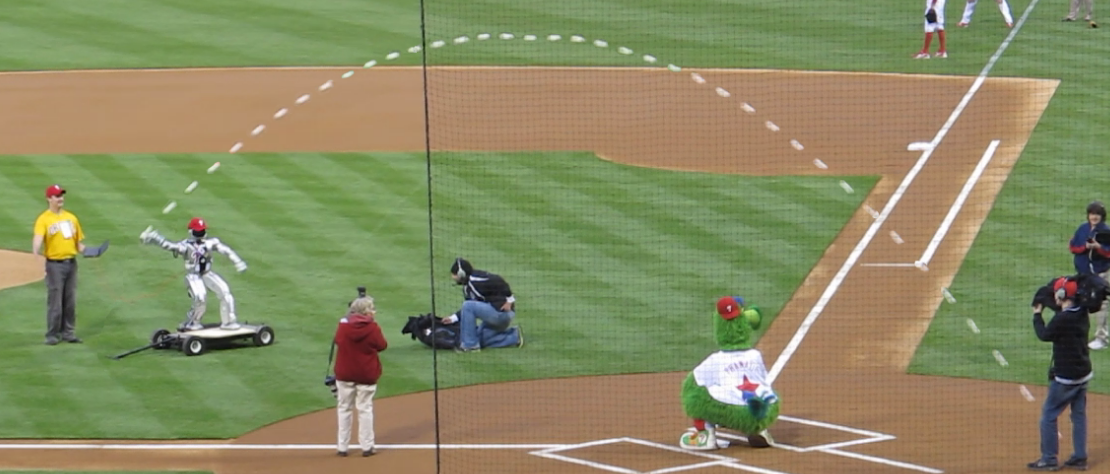
\includegraphics[width=1.0\textwidth]{./pix/philliesThrow.png}\\
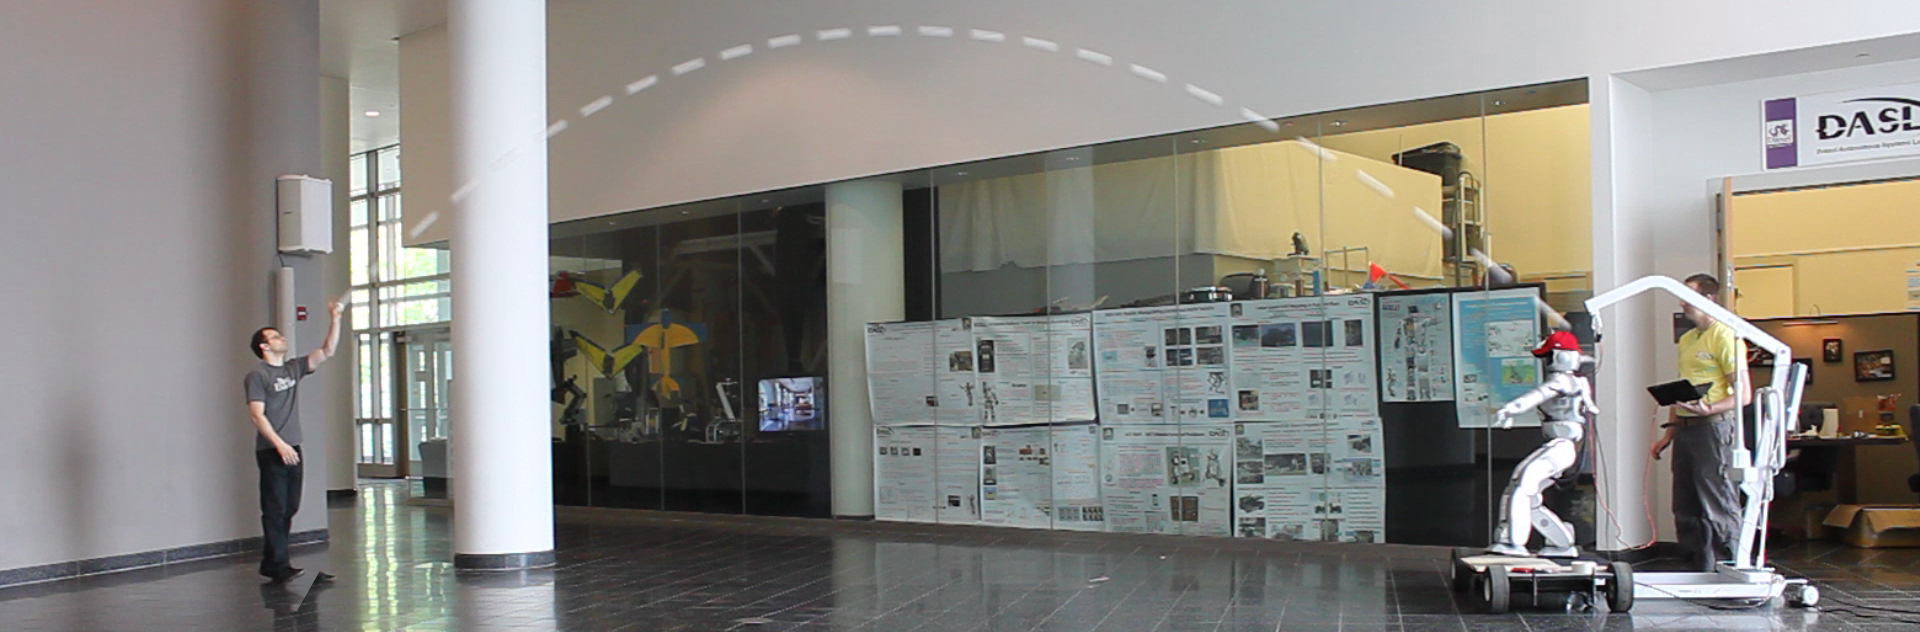
\includegraphics[width=1.0\textwidth]{./pix/preThrow2.png}
  \caption{(TOP) Pitch at Phillies Game.  (BOTTOM) Practice pitch at Drexel.  Frame overlay of the Hubo throwing overhand a distance of 10 m (32.8 feet) with a release angle of 40$^o$ and a tip speed of 10 $\frac{m}{s}$.  Captured at 20 fps with a shutter speed of 1/30 sec.  Each of the white dashes of in the image is the actual baseball as picked up by the video camera.}
  \label{fig:hubo-throw-test}
\end{figure}

An additional 2.5 $\frac{m}{s}$ was needed to give a proper throw.  
Borrowing from the GRASP Lab and their high powered pneumatic wrist on their PhillieBot, a spring loaded mechanism was added to Hubo's wrist, see Fig.~\ref{fig:hubo-spring}.
The addition of this mechanism allowed the robot to achieve an end-effector velocity magnitude of 10 $\frac{m}{s}$.
Fig.~\ref{fig:hubo-throw-test} shows a frame overlay of the the Hubo throwing a regulation baseball 10 m (32.8 feet).
Fig.~\ref{fig:hubo-throw} shows the same throw at Citizens Bank Park on April $28^{th}$, 2012.






\section{Conclusion}\label{sec:throw:conclusion}
	Throwing using the key-frame based method was the most reliable and successful.  
	The system was open-loop in respect to the location where it would throw the ball.
	This is why it over threw the ball during the real pitch, see Fig.~\ref{fig:hubo-throw-test}.
	The lessons learned when performing the throwing task is that
	\begin{enumerate}
		\item A unified algorithmic framework is needed for three tier testing
		\item Using such a framework the loop has to be closed on the ball's final location
		\item System for having a stable landing when taking a step
	\end{enumerate}

	Section~\ref{sec:hubo-ach} describes the unified framework that answer \#1 above.
	As stated before throwing is a full body locomotive task. 
	Section~\ref{sec:visuralServoing} closes the loop using visual methods.
	This shows how the unified algorithmic architecture can be used for visual servoing a full body locomotive tasks.
	This visual servoing example answer \#2 above.
	The use of active damping as seen in Section~\ref{sec:activedamping} allows the robot to land on the ground.
	This answers \#3 above.


